% !TEX program = xelatex
% 组会汇报：PSF 调查 2019–2024 跨年对齐（9 页，16:9）
% 编译：xelatex alignment_slides.tex（跑两遍以正确显示总页数）
\documentclass[aspectratio=169,11pt]{ctexbeamer}

\usetheme[progressbar=frametitle,numbering=fraction,block=fill]{metropolis}

\usepackage{booktabs}
\usepackage{graphicx}
\usepackage{tikz}
\usetikzlibrary{chains,positioning}
\usepackage{tcolorbox}
\tcbuselibrary{skins}

% ---------------------------------------------------------------- 配色与字体
\definecolor{ink}{HTML}{14213D}
\definecolor{muted}{HTML}{5A6472}
\definecolor{panel}{HTML}{F5F7FA}
\definecolor{border}{HTML}{E3E8EF}
\definecolor{accent}{HTML}{DD8452}
\definecolor{calm}{HTML}{4C72B0}
\definecolor{good}{HTML}{55A868}
\definecolor{warn}{HTML}{C44E52}

\setbeamercolor{frametitle}{bg=ink,fg=white}
\setbeamercolor{progress bar}{fg=accent,bg=ink!25}
\setbeamercolor{normal text}{fg=black!88}
\setbeamercolor{structure}{fg=calm}
\setbeamerfont{frametitle}{size=\large,series=\bfseries}
\setbeamertemplate{navigation symbols}{}

\setmonofont{Consolas}[Scale=0.92]

% ---------------------------------------------------------------- 版式组件
\newcommand{\lead}[1]{\vspace*{-1.2mm}{\color{muted}\small #1}\par\vspace{3.2mm}}
\newcommand{\code}[1]{{\ttfamily\upshape #1}}
\newcommand{\src}[1]{\vfill{\tiny\color{muted}#1}}

\newcommand{\kpi}[3]{%
  \begin{tcolorbox}[enhanced,colback=panel,colframe=panel,boxrule=0pt,arc=1.2mm,
      left=2.6mm,right=2mm,top=2mm,bottom=2mm,width=\linewidth,valign=center]
    {\color{#3}\bfseries\LARGE #1}\\[0.4mm]{\scriptsize\color{black!75}#2}
  \end{tcolorbox}}

\title{从 153 列到 110 列}
\subtitle{跨年对齐：人工映射、4B 模型与盘古 7B 的三种做法}
\author{汇报人：曾子睿}
\date{2026 年 11 月}

\begin{document}

% ---------------------------------------------------------------- 01 封面
\begin{frame}[plain]
  \vspace*{1mm}
  {\color{ink}\bfseries\fontsize{26}{30}\selectfont 153 列、110 列，与第三条路\par}
  \vspace{2mm}
  {\large\color{muted}跨年对齐：人工映射、4B 模型与盘古 7B 的三种做法\par}
  \vspace{3mm}

  \begin{center}
    \begin{tikzpicture}[x=1cm,y=1cm]
      \fill[panel] (0,0) rectangle (12.3,2.9);
      \node[anchor=west,font=\scriptsize,text=muted] at (0.5,2.45) {2019--2024 六份原始表};
      \node[anchor=west,font=\bfseries\large,text=ink] at (0.5,1.60) {42 个跨年共有列};
      \draw[->,line width=1.3pt,calm] (4.8,1.70) -- (7.0,1.70);
      \node[anchor=west,font=\bfseries\large,text=calm] at (7.2,1.70) {153（人工）};
      \node[anchor=west,font=\small,text=accent] at (7.2,1.05) {110（本地 4B 模型）};
      \node[anchor=west,font=\small,text=muted] at (7.2,0.45) {判断打平、归组失准（盘古 7B）};
      \node[anchor=west,font=\scriptsize,text=muted] at (0.5,0.62) {203,643 行 → 185,632 行};
    \end{tikzpicture}
  \end{center}

  \vfill
  {\small 汇报人：曾子睿 \hfill 2026 年 11 月}\\[1mm]
  {\tiny\color{muted}原始数据版权归 JetBrains / PSF 所有，此处只涉及对齐口径与脚本。}
\end{frame}

% ---------------------------------------------------------------- 02 成果
\begin{frame}{一页看清成果}
  \lead{人工路线交付完整总表；LLM 路线少 43 列，但两边都有的 105 列几乎逐格一致；盘古 7B 只到清洗层。}

  \begin{columns}[T,onlytextwidth]
    \column{0.235\textwidth}\kpi{153}{跨年共有列（原 42）}{calm}
    \column{0.235\textwidth}\kpi{382}{列名重命名}{good}
    \column{0.235\textwidth}\kpi{109,745}{取值统一记录}{accent}
    \column{0.235\textwidth}\kpi{185,632}{总表行数}{ink}
  \end{columns}

  \vspace{1.2mm}
  \begin{columns}[T,onlytextwidth]
    \column{0.54\textwidth}
      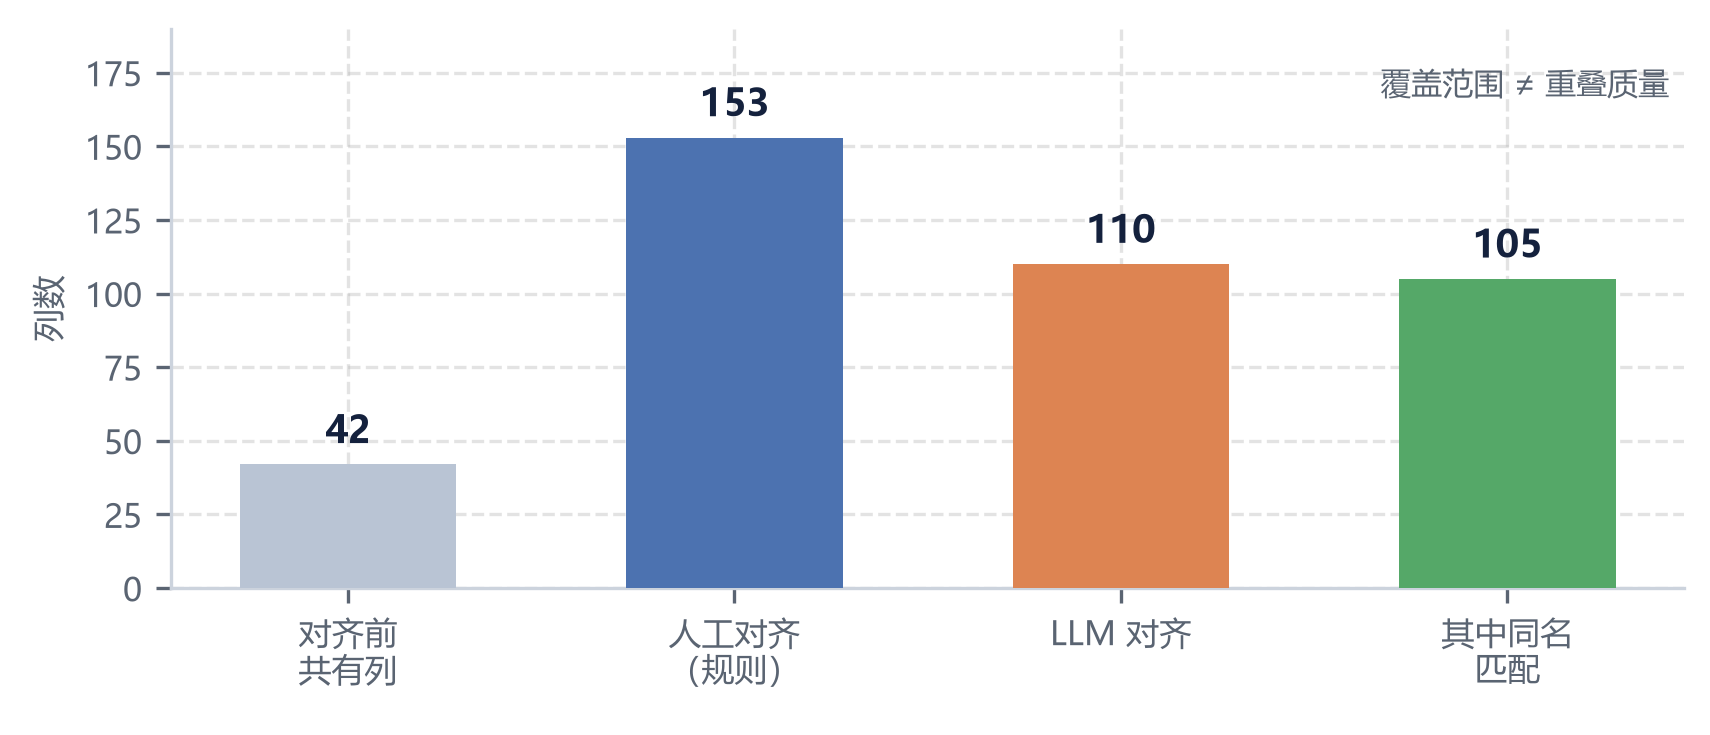
\includegraphics[width=\linewidth,height=0.28\textheight,keepaspectratio]{../figures/f1_coverage.png}
    \column{0.44\textwidth}
      {\scriptsize
        LLM：110 列 · 305 条重命名\\
        31 个同义簇 · 取值 5,217 条（单元格）\\
        105 列重叠，非空率差 $\geq$1pp：\textbf{0 条}\\
        同主题最大差 \textbf{0.1pp}（12 条对比）\\
        总行数 185,586，比人工少 46\\
        盘古 7B：8 对判定 100\%，单次 \textbf{13.7s}（4B 4.7s）
      }
  \end{columns}

  \src{来源：\code{aligned/alignment\_report.md}；\code{llm/reports/alignment\_report.md}；\code{llm/reports/parity\_report.md}；\code{pangu/reports/capability\_7b.json}}
\end{frame}

% ---------------------------------------------------------------- 03 手搓路径
\begin{frame}{手搓对齐：先归组，再改名，最后动取值}
  \lead{顺序不能反。先改列名再归组，前面的改动会被后一步覆盖。}

  \begin{center}
    \begin{tikzpicture}[start chain=going right,node distance=0.38cm,
        st/.style={on chain,draw=border,fill=panel,rounded corners=0.8mm,align=center,
            text width=1.95cm,inner sep=2pt,minimum height=1.25cm,font=\scriptsize},
        every join/.style={->,draw=border,line width=0.9pt}]
      \node[st]{\textbf{01}\\[0.6mm]文本归一};
      \node[st,join]{\textbf{02}\\[0.6mm]组路径重映射};
      \node[st,join]{\textbf{03}\\[0.6mm]列名统一};
      \node[st,join]{\textbf{04}\\[0.6mm]取值文案统一};
      \node[st,join]{\textbf{05}\\[0.6mm]取交集 153 列};
    \end{tikzpicture}
  \end{center}

  \vspace{2mm}
  {\scriptsize
    \begin{tabular}{@{}p{6.4cm}p{5.2cm}@{}}
      \toprule
      {\bfseries 改之前} & {\bfseries 改之后} \\
      \midrule
      \code{isolate.environments.Docker} & \code{environments.isolate.Docker} \\
      \code{what\_other\_language\_s...[Other]} & \code{other.lang.Other - Write In} \\
      \code{OS-provided Python (via apt-get...)} & \code{OS-provided Python} \\
      \bottomrule
    \end{tabular}
  }

  \vspace{1.6mm}
  {\scriptsize\color{muted}撞名先回退确定性归一，再撞才加 \code{\_\_dupN}；取值只合并同一选项的不同写法。}

  \src{来源：\code{aligned/alignment\_report.md}；\code{align\_survey.py}}
\end{frame}

% ---------------------------------------------------------------- 04 代价
\begin{frame}{手搓的代价：2019 一年改了 201 个列名}
  \lead{成本集中在第一次遇到新题型；后面五年加起来 181 条，维护靠同义词表逐年补。}

  \begin{center}
    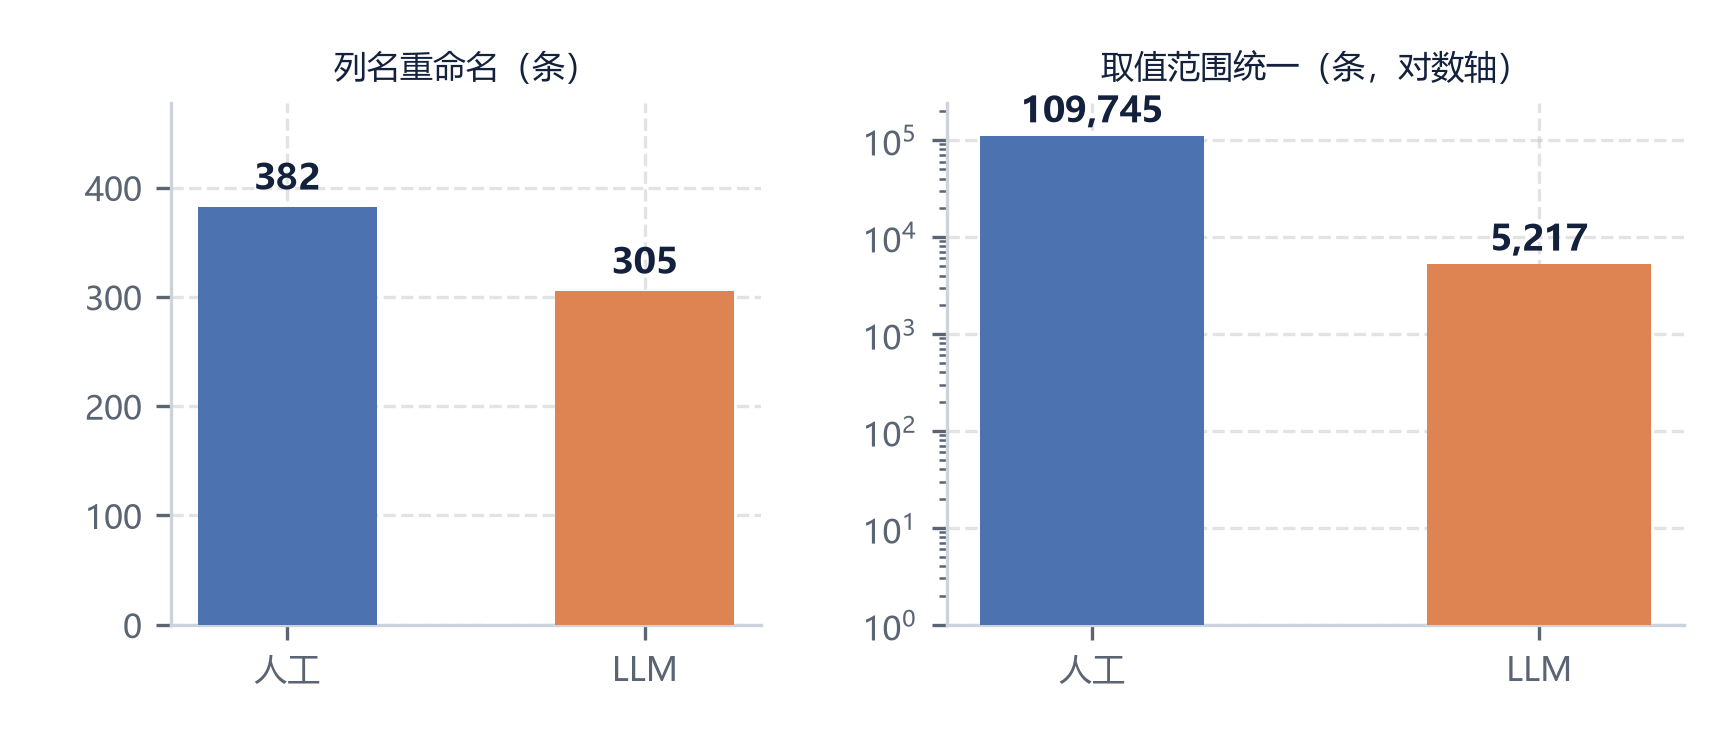
\includegraphics[width=0.88\textwidth,height=0.42\textheight,keepaspectratio]{../figures/f2_mapping_scale.png}
  \end{center}

  \vspace{0.4mm}
  {\scriptsize 分年重命名：2019 \textbf{201} · 31 · 48 · 43 · 25 · 34；2019 列名是整句问句，等于没有命名规范。}

  \src{来源：\code{aligned/alignment\_report.md} 分年统计；\code{llm/reports/alignment\_report.md} 校验提示}
\end{frame}

% ---------------------------------------------------------------- 05 LLM 路线
\begin{frame}{小模型：只动嘴，不动手}
  \lead{模型输出可校验的决策 JSON；执行、护栏、缓存都在 Python 里。}

  \begin{center}
    \begin{tikzpicture}[start chain=going right,node distance=0.5cm,
        st/.style={on chain,draw=border,fill=panel,rounded corners=0.8mm,align=center,
            text width=2.35cm,inner sep=2pt,minimum height=1.15cm,font=\scriptsize},
        every join/.style={->,draw=border,line width=0.9pt}]
      \node[st]{\textbf{01}\\[0.6mm]列画像\\（脱敏）};
      \node[st,join]{\textbf{02}\\[0.6mm]决策 JSON};
      \node[st,join]{\textbf{03}\\[0.6mm]确定性护栏};
      \node[st,join]{\textbf{04}\\[0.6mm]执行 / 缓存};
    \end{tikzpicture}
  \end{center}

  \vspace{2mm}
  \begin{columns}[T,onlytextwidth]
    \column{0.49\textwidth}
      {\scriptsize
        \textbf{304 个决策文件}：clean 149、align 130、stats 14，其余 11 个。\\
        首次全量约 30 分钟；命中缓存 2.7 分钟。
      }
    \column{0.49\textwidth}
      {\scriptsize
        组路径 20 处改道、选项同义簇 31 个；\\
        逐对判定 162 对（接受 34 对），取值统一 5,217 条——\\
        4B 不生成写法，只答“是不是同一个”。
      }
  \end{columns}

  \vspace{1.8mm}
  {\scriptsize\color{muted}
    护栏：Yes/No 禁改道版本路径 · 题型冲突拒合 · 选项指纹 Jaccard $\geq$0.2 · 结构不得重复拼接 · 簇 $\leq$4 且 $\leq$50\%。}

  \src{来源：\code{llm/README.md}；\code{llm/decisions/} 计数；\code{llm/reports/alignment\_report.md}}
\end{frame}

% ---------------------------------------------------------------- 06 对账
\begin{frame}{对账：两条能对账，第三条只能对到列}
  \lead{第三条没有对齐产物，只能在清洗语义这一层逐列比；名字对了、语义错了更难发现。}

  \begin{center}
    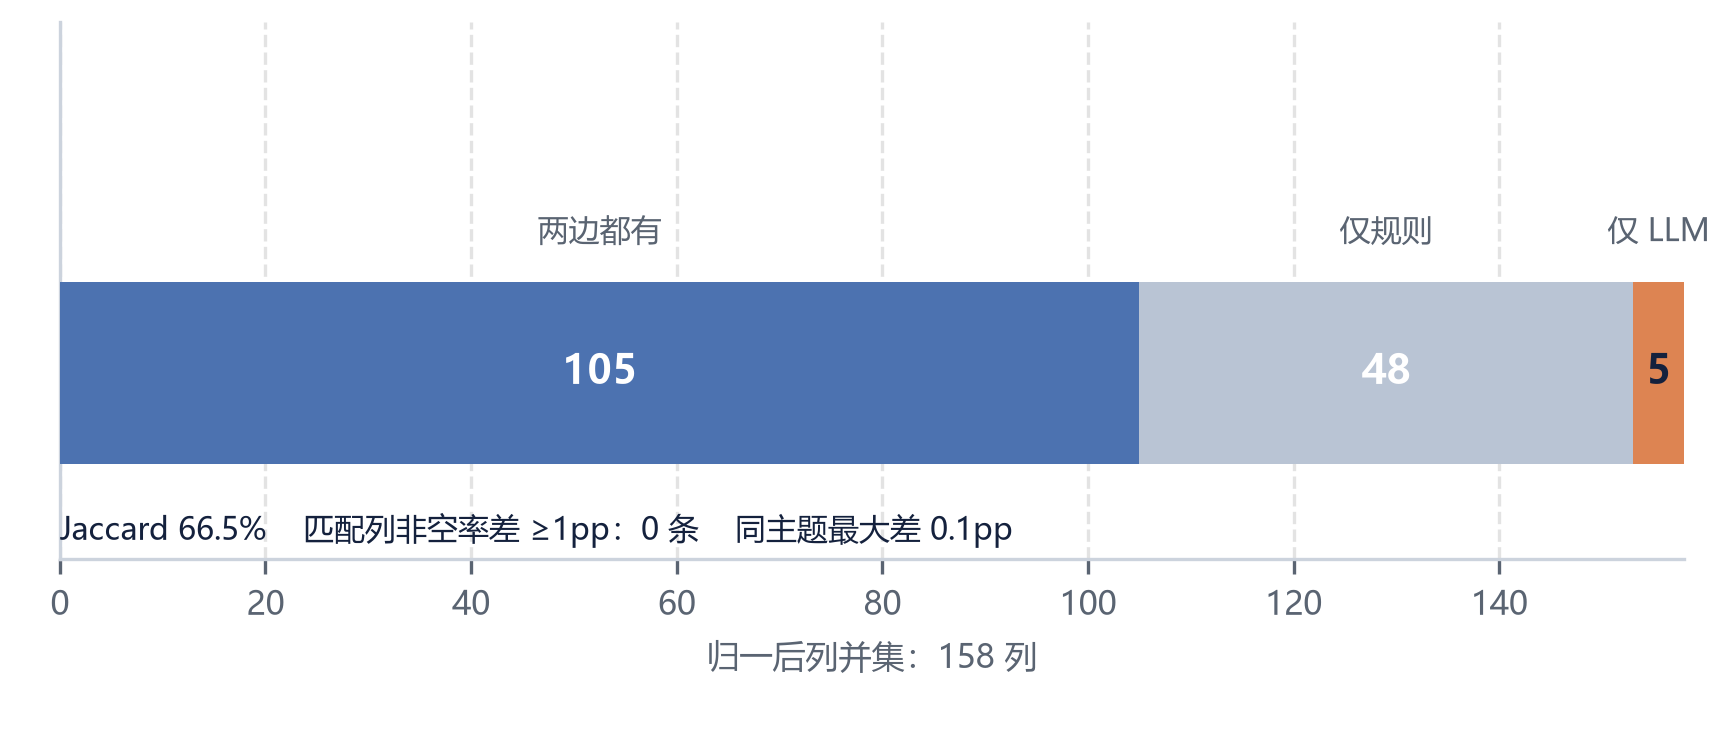
\includegraphics[width=0.90\textwidth,height=0.30\textheight,keepaspectratio]{../figures/f3_parity.png}
  \end{center}

  \begin{columns}[T,onlytextwidth]
    \column{0.47\textwidth}
      {\scriptsize
        并集 158 = 105 匹配 + 48 仅人工 + 5 仅 LLM；Jaccard 66.5\%。\\
        105 个匹配列非空率差 $\geq$1pp：\textbf{0 条}；同主题最大差 0.1pp。\\
        2023/2024 映射未进提示词，105 是留出成绩。
      }
    \column{0.50\textwidth}
      {\scriptsize
        改造前的反例：\code{is.python.main} 被映射成 \code{ide.python\_version}。\\
        路径合法，但语义是“是否以 Python 为主”，不是版本；\\
        2019 年五个来源列并成一组，四个版本列变 \code{\_\_dup}。\\
        现在取值指纹护栏直接拒掉。
      }
  \end{columns}

  \src{来源：\code{llm/reports/parity\_report.md}；\code{llm/reports/alignment\_report.md}}
\end{frame}

% ---------------------------------------------------------------- 07 第三条路
\begin{frame}{第三条路：盘古 7B 走到了哪一步}
  \lead{同一条管线、同一套提示词只换模型：8 对边界样本判断打平，成本高一个量级。}

  \begin{center}
    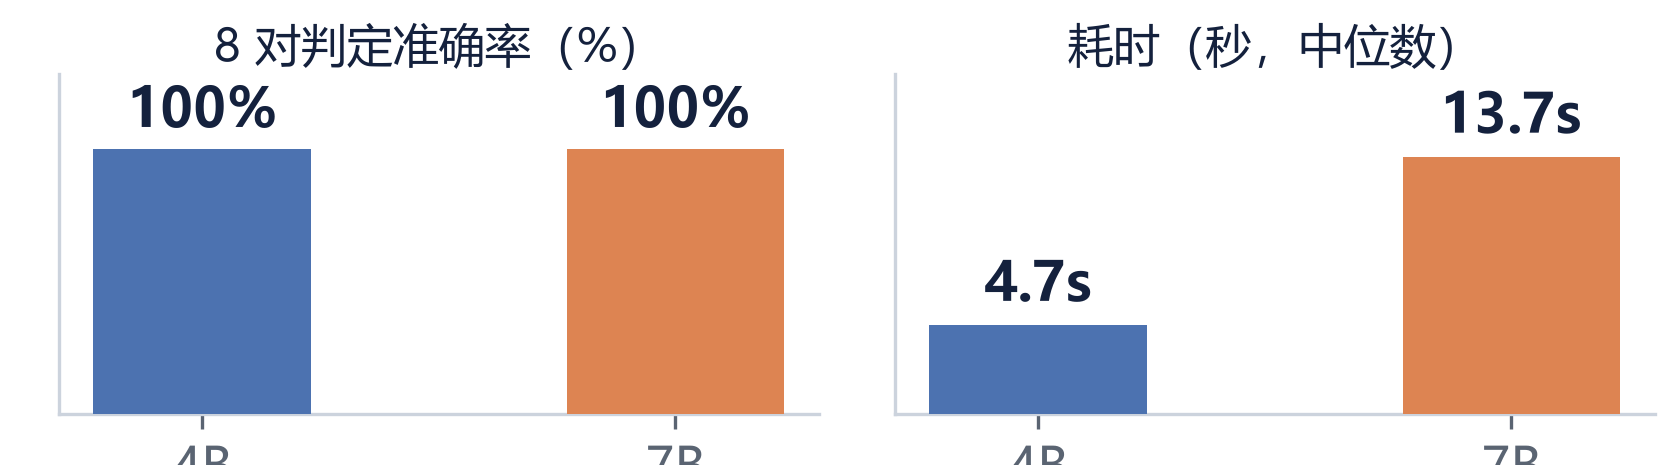
\includegraphics[width=0.70\textwidth]{../figures/f4_capability.png}
  \end{center}

  {\scriptsize
    \textbf{选型}：Q4\_K\_M 4.59 GiB 全 GPU、57 tok/s；2.0 最小档 40.7 GiB，本机装不下。\\
    \textbf{不兼容}：\code{format=json} 报 400、\code{think=false} 空转，每列多 300--400 token 推理正文。\\
    \textbf{同口径成本}（2019 清洗 156 列）：每列 407 token 对 55（\textbf{7.4 倍}），纯推理 6.6 s 对 0.7 s（\textbf{9 倍}）。\\
    \hspace*{18mm}墙钟跨度 127 分钟里 112 分钟是两次调用之间的空档，不算模型开销。
  }

  \src{来源：\code{pangu/reports/capability\_7b.json}；\code{pangu/reports/hardware.json}；成本取 \code{pangu/reports/benchmark.md}（2026-10-29 21:20 快照）}
\end{frame}

% ---------------------------------------------------------------- 08 扩样对账
\begin{frame}{样本扩到 138 列：题型对得上，题目组对不上}
  \lead{8 对样本看不出差别，换成 2019 年两侧都判过的 138 列，三项判定逐列比。}

  \begin{columns}[T,onlytextwidth]
    \column{0.41\textwidth}
      {\scriptsize
        \begin{tabular}{@{}lrr@{}}
          \toprule
          {\bfseries 判定项} & {\bfseries 一致} & {\bfseries 占比} \\
          \midrule
          kind（题型）    & 133 & 96.4\% \\
          option（选项名）& 98  & 71.0\% \\
          group（题目组） & 7   & 5.1\% \\
          \midrule
          三项全同        & 7   & 5.1\% \\
          \bottomrule
        \end{tabular}
      }

      \vspace{2.2mm}
      {\scriptsize\color{muted}只读决策缓存；未覆盖的列不参与分母。}

    \column{0.57\textwidth}
      {\scriptsize
        \textbf{组名基数}：138 列上 4B 给 40 个 group，7B 给 91 个。\\
        \textbf{不是看不见兄弟列}：4 列一批的 109 列一致率 6.4\%，1 列一批的 21 列全 0\%。\\
        \textbf{只发生在 2019}：2020 表头自带组路径，两个前缀各 5 列都是 5/5 同组；\\
        2019 的表头是「选项:问句」，没有锚点可抄。\\
        \textbf{一个例子}：Big Data 工具题 9 个选项，4B 归 1 组，7B 拆成 8 组。\\
        \textbf{代码兜住结构}：\code{\_stabilize\_2019\_groups} 按问句多数票并组，组名退化成某个选项名。
      }
  \end{columns}

  \src{来源：\code{pangu/reports/semantics\_compare\_2019.md}；\code{pangu/reports/group\_follow\_2020.json}；\code{llm/llm\_survey/clean\_stage.py}}
\end{frame}

% ---------------------------------------------------------------- 09 结论
\begin{frame}{结论：人工交付，4B 出候选，7B 只做仲裁}
  \lead{三条路各有位置；模型写得最顺的差异解释，反而最不能直接信。}

  \begin{columns}[T,onlytextwidth]
    \column{0.47\textwidth}
      {\bfseries\color{good} 能交给 4B}\\[1.5mm]
      {\scriptsize
        \begin{itemize}\setlength{\itemsep}{0.8mm}
          \item 逐对判同题、判同义：只答 a/b，聚簇交给代码。
          \item 新一年的组路径候选，人工只审 diff。
          \item 对账差异草稿，数字由脚本回填。
        \end{itemize}}
    \column{0.49\textwidth}
      {\bfseries\color{warn} 必须留给人}\\[1.5mm]
      {\scriptsize
        \begin{itemize}\setlength{\itemsep}{0.8mm}
          \item 命名终审：候选路径与选项写法由人工词表定。
          \item 删行删列：宁可少删，不能误删。
          \item 数字与结论：叙述可润色，数值以 CSV 为准。
        \end{itemize}}
  \end{columns}

  \vspace{1.8mm}
  {\scriptsize\textbf{盘古 7B}：kind 对得上（96.4\%），组路径对不上（5.1\%）；token 7.4 倍、无 JSON 约束、推理关不掉——只对少数高风险判断做二次确认。}

  \vspace{1.2mm}
  {\scriptsize\color{muted}
    下一步：给跨年改名题补名称证据（\code{develop.for.cloud}、\code{orm}、\code{unittesting} 仍判 \code{keep}）；被拒映射进人工确认队列；盘古若要进主线，先解决 2019 的组路径锚点与推理正文抑制这两件事。}

  \src{谢谢大家！}
\end{frame}

\end{document}
